\documentclass[a4paper,11pt,spanish,leqno]{article}
\usepackage{amssymb}
\usepackage[utf8]{inputenc}
\usepackage{hyperref}
\usepackage{graphicx}
\title{Tarea 8}
\author{Juan Velasco Izquierdo}


\begin{document}
\maketitle
\paragraph{}\textbf{Sea el método numérico $y_{n+2}-y_{n} = h\frac{2}{3} (f_{n+2} + f_{n+1} + f_{n+2})$, identificar la región de estabilidad del método lineal multipaso y decidir si es A-Estable.}

\paragraph{}Dado que nos encontramos ante un método lineal multipaso (MLM), la primera forma que tenemos de ver cómo es la región de estabilidad es usando el polinomio de estabilidad $\Pi(r,z)$. Para ello primero tenemos que identificar el primer y el segundo polinomio característicos. Vamos a ver los tres polinomios.

$\rho(\xi)=\xi^2 + 1$

$\sigma(\xi)=\frac{2}{3}\xi^2 + \frac{2}{3}\xi + \frac{2}{3}$

$\Pi(r,z)=\rho(r) - z\sigma(r) = r^2 - 1 - \frac{2}{3}zr^2 - \frac{2}{3}zr - \frac{2}{3}z = (1-\frac{2}{3}z)r^2 - (\frac{2}{3}z)r - (1+\frac{2}{3}z)$

\paragraph{}La primera forma de ver si es A-Estable y determinar su región de estabilidad $D$ es encontrar las raíces $r(z)$ del polinomio $\Pi(r,z)$ tales que $|r(z)|<1$. En nuestro caso es bastante difícil obtener estas raíces por lo que vamos a utilizar el segundo método.

\paragraph{}El segundo método consiste en observar la frontera de al región de estabilidad $\partial D$, el cual está contenido en $F:=\{z \in \mathbb{C}:$ existe una raíz de $\Pi(.,z)$de módulo $1\}$. Sea $z\in F$, este $z$ viene determinado por:

$z = \frac{\rho(e^{i\theta})}{\sigma(e^{i\theta})}$, con $0\leq \theta < 2\pi$

Por lo tanto $F$ es la imagen de una curva cerrada que separa $\mathbb{C}$ en dos regiones disjuntas
$\mathbb{C} \backslash F = A_1 \sqcup A_2$, y por tanto o bien $\partial D \subseteq A_1$ o bien $\partial D \subseteq A_2$. Para ver cual caso se da simplemente hay que estudiar un punto.

\paragraph{}Vamos a empezar viendo como es $F$ usando como son los elementos del mismo. Pero primero vamos a ver un par de igualdades que usaremos en el desarrollo:

$(1)\ e^{ni\theta} = \cos(n\theta) +  \sin(n\theta)$

$(2)\ ie^{i\theta} = i\cos(n\theta) - \sin(\theta)$

$(3)\ \sin(2\theta) = 2\sin(\theta)\cos(\theta)$

$(4)\ \cos(2\theta) = \cos^2(\theta) - \sin^2(\theta)$

$(5)\ \sin^2(\theta) + \cos^2(\theta) = 1$
\\\\
Pasemos al desarrollo:
\\\\\
$z = \frac{\rho(e^{i\theta})}{\sigma(e^{i\theta})} = \frac{e^{2i\theta - 1}}{\frac{2}{3}e^{2i\theta} + \frac{2}{3}e^{i\theta} + \frac{2}{3}} = $

Usando (1)  

$ = \frac{\cos(2\theta) + i\sin(2\theta) - 1}{\frac{2}{3}(\cos(2\theta) + i\sin(2\theta) + \cos(\theta) + i\sin(\theta) + 1)} =$

Usando (3), (4) y (5)

$ = \frac{3}{2}\frac{\cos^2(\theta) - \sin^2(\theta) + i2\sin(\theta)\cos(\theta) - \sin^2(\theta) - \cos^2(\theta)}{\cos^2(\theta) - \sin^2(\theta) + i2\sin(\theta)\cos(\theta) + \cos(\theta) + i\sin(\theta) + \sin^2(\theta) + \cos^2(\theta)} = $

$ = \frac{3}{2} \frac{-2\sin^2(\theta) + 2i\sin(\theta)\cos(\theta)}{2\cos^2(\theta) + 2i\cos(\theta)\sin(\theta) + \cos(\theta) + i\sin(\theta)} = \frac{3}{2}\frac{\sin(\theta)(-\sin(\theta) + i\cos(\theta))}{\cos(\theta)(\cos(\theta) + i\sin(\theta)) +\frac{1}{2}(\cos(\theta) + i\sin(\theta))} =$

Usando (1) y (2)

$ = \frac{3}{2}\frac{\sin(\theta)ie^{i\theta}}{\cos(\theta)e^{i\theta} + \frac{1}{2}e^{i\theta}} = \frac{3\sin(\theta)}{2\cos(\theta) + 1}i$

\paragraph{}Por tanto:

$F = \{z \in \mathbb{C}: z = \frac{3\sin(\theta)}{2\cos(\theta) + 1}i , \theta \in [0,2\pi] \}$

Podemos intuir que $F$ es un segmento en el eje vertical, pero hemos usado Matlab para realizar una gráfica del mismo, la cual mostramos a continuación.

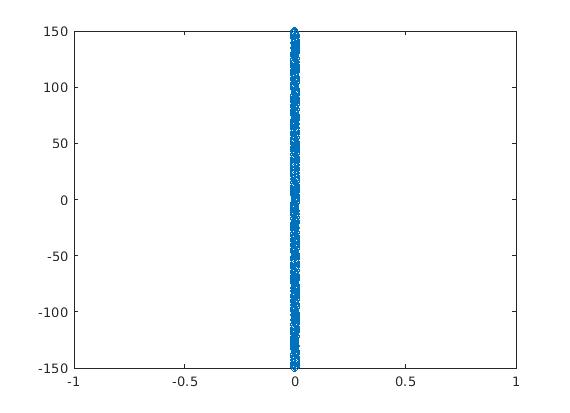
\includegraphics[scale=0.5]{Entrega8.jpg}

Esto confirma nuestras sospechas y por tato $D$ está en el $int(F)$ y por tanto $D= \emptyset $ o bien $D=\mathbb{C} \backslash F$

Para ver esto simplemente tenemos que coger un punto en $\mathbb{C}_{\_}$ y ver si sus raíces tienen módulo menor que 1. Si sucede esto $D=\mathbb{C} \backslash F$ y además es A-estable.

$\Pi(r,-\frac{3}{2}) = 2r^2 + r = r(2r + 1)$ Por lo tanto $r_1(-\frac{3}{2})=0$ y $r_2(-\frac{3}{2})=-\frac{1}{2}$, ambas de módulo menor que 1.

Concluimos pues que \textbf{el método es A-estable} y \textbf{$D=\mathbb{C} \backslash F$}.
\end{document}. 
